\documentclass{article}
\usepackage[utf8]{inputenc}
\usepackage{geometry}
\usepackage{amsmath}
\usepackage{url}
\usepackage[utopia]{mathdesign}
\usepackage{lipsum}  
\usepackage{lmodern}
\usepackage{listings}
\usepackage{tikz}
\usetikzlibrary{arrows.meta, positioning}

 \geometry{
 a4paper,
 total={170mm,257mm},
 left=20mm,
 top=20mm,
 }
 \usepackage{graphicx}
 \usepackage{titling}

 \title{Report \#4}
\author{GU JUN}
\date{November 19, 2024}
 
 \usepackage{fancyhdr}
\fancypagestyle{plain}{%  the preset of fancyhdr 
    \fancyhf{} % clear all header and footer fields
%    \fancyfoot[R]{\includegraphics[width=5cm]{}}
    \fancyfoot[L]{\today}
    \fancyhead[L]{Analytical Mechanics 80848\#1}
    \fancyhead[R]{HIRAI SHINCHI}
}
\makeatletter
\renewcommand{\maketitle}{%
  \newpage
  \null
  \vskip 1em%
  \begin{center}%
  \let \footnote \thanks
    {\LARGE \@title \par}%
    \vskip 1em%
    %{\large \@date}%
  \end{center}%
  \par
  \vskip 1em}
\makeatother


\begin{document}

\maketitle

\noindent\begin{tabular}{@{}ll}
    Student & \theauthor\\
    ID number & 6132230056 \\
\end{tabular}

\section*{Problem Statement}
Simulate the motion of a 2DOF closed link mechanism under PID
control. PID control is applied to active joints 1 and 3. Use
appropriate values of geometrical and physical parameters of the
manipulator.
\begin{figure}[h!]
  \centering
  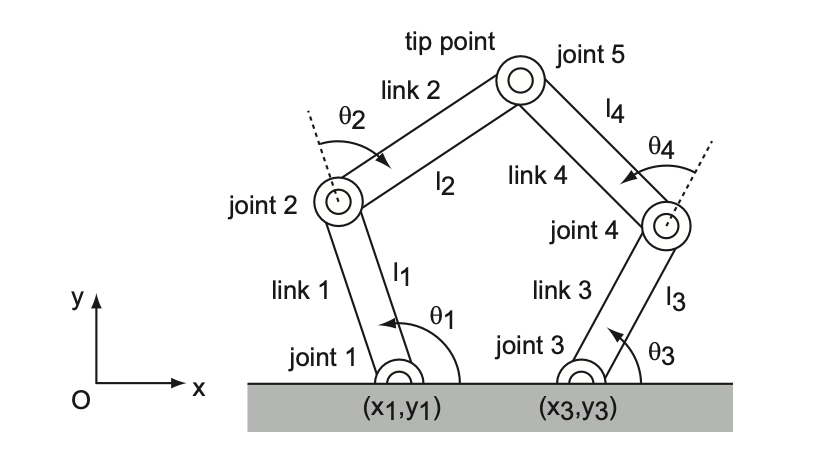
\includegraphics[width=0.8\textwidth]{assets/model.png}
  \caption{Model of the 2DOF closed link mechanism}
  \label{fig:model-2dof}
\end{figure}

\section*{PID Control}
The control law for the PID controller is given by:

\[
\tau = -K_p \cdot \text{e} - K_d \cdot \omega - K_i \cdot \int \text{e} \, dt
\]

where:
\begin{itemize}
  \item \(\tau\) is the control input (torque) applied to the joints.
  \item \(K_p\) is the proportional gain.
  \item \(K_d\) is the derivative gain.
  \item \(K_i\) is the integral gain.
  \item \(\text{e}\) is the difference between the desired and actual position.
  \item \(\omega\) is the angular velocity of the joint.
  \item \(\text{integral}\) is the accumulated error over time.
\end{itemize}
The PID controller aims to minimize the error by adjusting the control input \(\tau\) based on the proportional, derivative, and integral terms. The proportional term \(K_p \cdot \text{e}\) corrects the error based on the current difference between the desired and actual position. The derivative term \(K_d \cdot \omega\) provides a damping effect by considering the rate of change of the error, thus reducing overshoot and oscillations. The integral term \(K_i \cdot \int \text{e} \, dt\) accounts for the accumulated error over time, ensuring that the steady-state error is minimized.

\newpage

\subsection*{Matlab Code}
Based on the given example code and the PID control law, the following Matlab code was implemented to simulate the motion of the 2DOF closed link mechanism under PID control.

\begin{verbatim}
  function dotq = closed_mechanism_2DOF_PID_params (t, q, robot, thetad, Kp, Ki, Kd)
  % equation of motion of 2DOF closed mechanism under PD control
      % disp(num2str(t,"%8.6f"));
      persistent alpha
      if isempty(alpha)
          alpha = 1000;
      end
      
      theta = q(1:4);
      omega = q(5:8);
      integral = q(9:10);
      
      dottheta = omega;
      
      theta12 = theta(1:2); omega12 = omega(1:2);
      theta34 = theta(3:4); omega34 = omega(3:4);
      robot.left_arm = robot.left_arm.joint_angles (theta12, omega12);
      robot.right_arm = robot.right_arm.joint_angles (theta34, omega34);
      
      J12 = robot.left_arm.Jacobian;
      J34 = robot.right_arm.Jacobian;    
      [ Q12x, Q12y ] = robot.left_arm.Hessian;
      [ Q34x, Q34y ] = robot.right_arm.Hessian;
      
      [inertia_matrix_12, torque_vector_12] = robot.left_arm.inertia_matrix_and_torque_vector;
      [inertia_matrix_34, torque_vector_34] = robot.right_arm.inertia_matrix_and_torque_vector;
      
      R = robot.left_arm.tip_point - robot.right_arm.tip_point;
      dotR = J12*omega12 - J34*omega34;
  
      C = [ omega12'*Q12x*omega12 - omega34'*Q34x*omega34; ...
            omega12'*Q12y*omega12 - omega34'*Q34y*omega34 ];
      C = C + 2*alpha*dotR + (alpha^2)*R;
      error1 = theta(1) - thetad(1);
      error2 = theta(3) - thetad(2);
      tau_left  = [ -Kp(1)*error1 - Kd(1)*omega(1) - Ki(1) * integral(1); 0 ];
      tau_right = [ -Kp(2)*error2 - Kd(2)*omega(3) - Ki(2) * integral(2); 0 ];
      
      A = [ inertia_matrix_12,        zeros(2,2), -J12'; ...
                   zeros(2,2), inertia_matrix_34,  J34'; ...
                         -J12,               J34, zeros(2,2) ];
      b = [ torque_vector_12 + tau_left; ...
            torque_vector_34 + tau_right; ...
            C ];
      
      p = A \ b;
      dotomega = p(1:4);
      
      dotq = [dottheta; dotomega; error1; error2];
  end
  end
\end{verbatim}

To achieve PID control, I add the $K_i$ term as the new parameter and add \textbf{integral} to the state description \textbf{q}. The error is calculated as the difference between the desired and actual position. The control input \(\tau\) is then computed based on the PID control law. The derivative of the state vector \textbf{q} is returned as the output.

\subsection*{PID Parameters}
After some trial and error, the following PID parameters were chosen to achieve stable and accurate control of the 2DOF closed link mechanism:
\begin{table}[h!]
  \centering
  \begin{tabular}{|c|c|}
    \hline
    \(K_p^T\) & (3.0, 3.0) \\
    \(K_i^T\) & (0.8, 0.8) \\
    \(K_d^T\) & (0.5, 0.5) \\
    \hline
  \end{tabular}
  \caption{PID Parameters}
  \label{tab:pid-params}
\end{table}
\section*{Simulation Results}

\begin{figure}[h!]
  \centering
  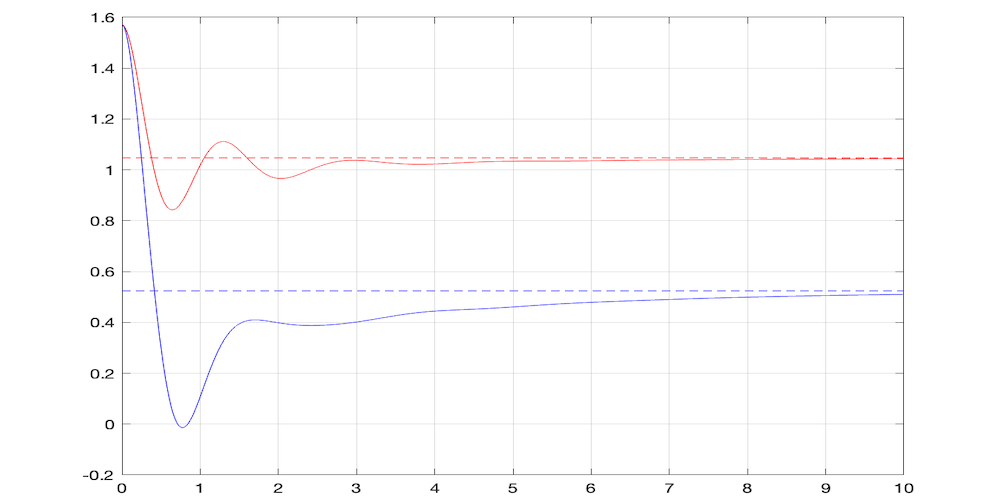
\includegraphics[width=0.4\textwidth]{assets/closed_mechanism_2DOF_PID_angles.png}
  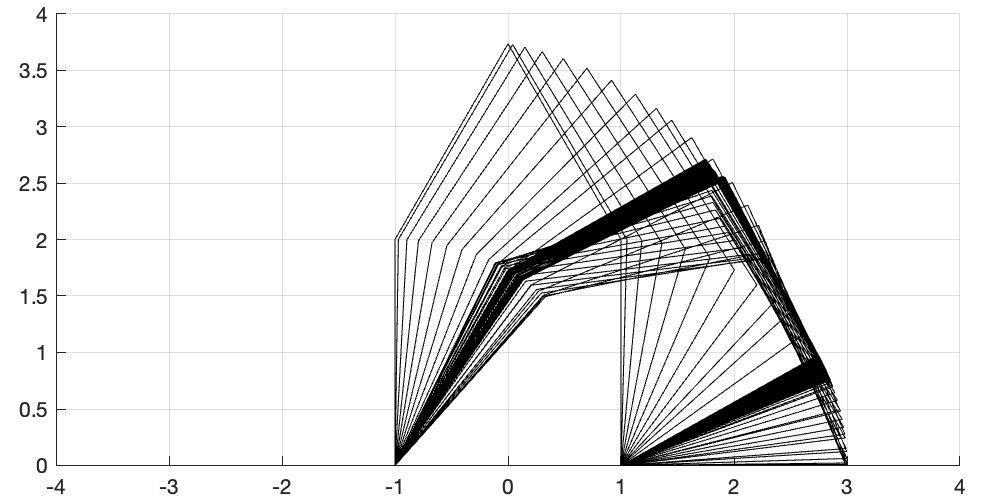
\includegraphics[width=0.4\textwidth]{assets/closed_mechanism_2DOF_PID_draw.png}
  \caption{2DOF Closed Link Mechanism under PID Control, left side: joint angles, right side: mechanism drawing}
  \label{fig:2dof-closed-link-mechanism}
\end{figure}

As shown in Figure \ref{fig:2dof-closed-link-mechanism}, the 2DOF closed link mechanism under PID control exhibits stable and accurate motion than normal PD control. The joint angles converge to the desired values, and the mechanism follows the desired trajectory effectively. The chosen PID parameters provide a good balance between tracking performance and stability, resulting in smooth and precise control of the mechanism.
A video demonstration of the 2DOF closed link mechanism under PID control can be viewed at the following link:

\url{https://mushroomspace.notion.site/video-for-report-3-1436031a26338051985ec594ad084aa9}

\end{document}
